\chapter{Firmware Project}\label{ch:software-project}

	\section{Microcontroller programming basics}\label{ssec:microcontroller-programming-basics}
		A microcontroller code is composed basically of two parts:
		
		\begin{itemize}
			\item \textit{Setup: } This part of the code is only executed once, as the name may indicate, it is used to set properties, configure timers, inputs and other features of the hardware.
			\item \textit{Loop: } This part of the code is executed continuously or until some condition is reached. 
		\end{itemize}
		
		\par
		
		Other important component of a microcontroller code are interruptions. It is possible to interrupt the standard execution of a program when an event happens, or as it is more common to say, when an event triggers a interruption. This event may be a timer overflow, an event triggered by an input change among other things. Interrupt routines are really useful when working with intrumentation and timers, because using interruptions it is feasible to meet real-time requirements in a project \cite{mukaro1999microcontroller}.
		
	\section{Code Map}\label{sec:microcontroller-code-map}
	
	The Figure \ref{fig:microCode} show a functional map of the microcontroller code.
	
	\begin{figure}[htbp]
		\centering
		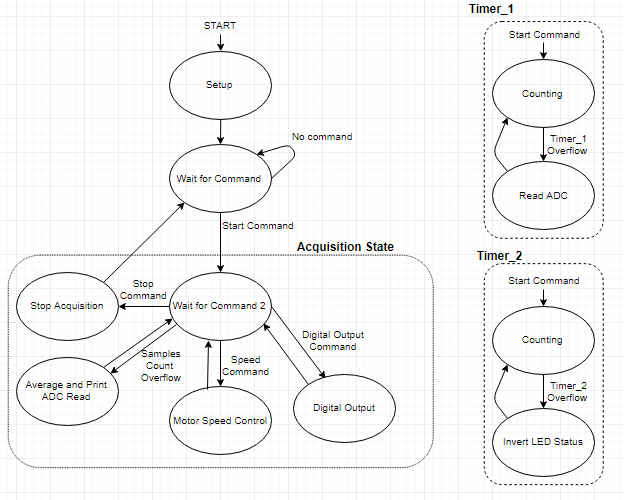
\includegraphics[width=.8\textwidth]{figuras/fig-microCodeMap}
		\caption{Microcontroller Code Map}
		\label{fig:microCode}
	\end{figure}
	
	
	As soon as the microcontroller is turned on it enters in the \textit{Setup}, on this part the following things are setted:
	\begin{itemize}
		\item \textit{Acquisition Timer:} Timer max count value is setted and an interruption service routine is appointed, this timer is used for the analog sampling/reading function.\label{itm:mcu-prog-timer1}
		\item \textit{LED Timer:} Same thing done for \textit{Acquisition Timer}is done for \textit{LED Timer}, this timer controls the blinking frequency of the MCU debug LED.\label{itm:mcu-prog-timer2}
		\item \textit{Serial Port: } The serial port baud rate is defined and the serial port is opened.\label{itm:mcu-prog-serial-port}
		\item \textit{Port mapping: } The port mapping is done, \textit{i.e.} digital I/O ports are defined as inputs (high impedance) or as outputs (low impedance) and the analog ports are setted.\label{itm:mcu-prog-port}
	\end{itemize}
	
	After setting up, the code enters in a state in which it waits for a command that can be from three different groups. This commands are coded into ASCII characters \cite{ascii}. Table \ref{table:ascii-commands} shows all proposed commands.

	\begin{table}[h!]
		\begin{tabular}{|l|l|l|l|l|l|}
		\hline
		\textbf{ASCII} & \textbf{Command} & \textbf{ASCII} & \textbf{Command} & \textbf{ASCII} & \textbf{Command} \\ \hline
		32 & Print Version & 65 &  & 98 & PWM 1 - DT 92\% \\ \hline
		33 & Filter Read & 66 &  & 99 & PWM 1 - DT 96\% \\ \hline
		34 & One Read & 67 &  & 100 & PWM 1 - DT 100\% \\ \hline
		35 & DOUT - Reset & 68 &  & 101 & PWM 2 - DT 0\% \\ \hline
		36 & DOUT 1 - ON & 69 &  & 102 & PWM 2 - DT 4\% \\ \hline
		37 & DOUT 1 - OFF & 70 &  & 103 & PWM 2 - DT 8\% \\ \hline
		38 & DOUT 2 - ON & 71 &  & 104 & PWM 2 - DT 12\% \\ \hline
		39 & DOUT 2 - OFF & 72 &  & 105 & PWM 2 - DT 16\% \\ \hline
		40 & DOUT 3 - ON & 73 &  & 106 & PWM 2 - DT 20\% \\ \hline
		41 & DOUT 3 - OFF & 74 &  & 107 & PWM 2 - DT 24\% \\ \hline
		42 &  & 75 & PWM 1 - DT 0\% & 108 & PWM 2 - DT 28\% \\ \hline
		43 &  & 76 & PWM 1 - DT 4\% & 109 & PWM 2 - DT 32\% \\ \hline
		44 &  & 77 & PWM 1 - DT 8\% & 110 & PWM 2 - DT 36\% \\ \hline
		45 &  & 78 & PWM 1 - DT 12\% & 111 & PWM 2 - DT 40\% \\ \hline
		46 &  & 79 & PWM 1 - DT 16\% & 112 & PWM 2 - DT 44\% \\ \hline
		47 &  & 80 & PWM 1 - DT 20\% & 113 & PWM 2 - DT 48\% \\ \hline
		48 &  & 81 & PWM 1 - DT 24\% & 114 & PWM 2 - DT 52\% \\ \hline
		49 &  & 82 & PWM 1 - DT 28\% & 115 & PWM 2 - DT 56\% \\ \hline
		50 &  & 83 & PWM 1 - DT 32\% & 116 & PWM 2 - DT 60\% \\ \hline
		51 &  & 84 & PWM 1 - DT 36\% & 117 & PWM 2 - DT 64\% \\ \hline
		52 &  & 85 & PWM 1 - DT 40\% & 118 & PWM 2 - DT 68\% \\ \hline
		53 &  & 86 & PWM 1 - DT 44\% & 119 & PWM 2 - DT 72\% \\ \hline
		54 &  & 87 & PWM 1 - DT 48\% & 120 & PWM 2 - DT 76\% \\ \hline
		55 &  & 88 & PWM 1 - DT 52\% & 121 & PWM 2 - DT 80\% \\ \hline
		56 &  & 89 & PWM 1 - DT 56\% & 122 & PWM 2 - DT 84\% \\ \hline
		57 &  & 90 & PWM 1 - DT 60\% & 123 & PWM 2 - DT 88\% \\ \hline
		58 &  & 91 & PWM 1 - DT 64\% & 124 & PWM 2 - DT 92\% \\ \hline
		59 &  & 92 & PWM 1 - DT 68\% & 125 & PWM 2 - DT 96\% \\ \hline
		60 &  & 93 & PWM 1 - DT 72\% & 126 & PWM 2 - DT 100\% \\ \hline
		61 &  & 94 & PWM 1 - DT 76\% & 127 &  \\ \hline
		62 &  & 95 & PWM 1 - DT 80\% &  &  \\ \hline
		63 &  & 96 & PWM 1 - DT 84\% &  &  \\ \hline
		64 &  & 97 & PWM 1 - DT 88\% &  &  \\ \hline
		\end{tabular}
		\caption{ASCII Commands Reference}
		\label{table:ascii-commands}
	\end{table}


	Each group of commands will lead to a specific block described in Figure \ref{fig:microCode}.

	\begin{itemize}
		\item \textit{Digital Output Control:} As mentioned in Section \ref{sssec:lower-level-hardware-interfaces}, there are three digital outputs on the circuit board. Hence, there will be two commands for each digital channel (on and off) plus a command to turn all the digital outputs off. 
		\item \textit{Analog Output Control:} Commands from this block will set the duty cycle for the MCU PWM outputs that will be converted to analog outputs, as explained in Section \ref{sec:speed-reference-output-channel}.
		\item \textit{Acquisition State: } There is only one command that will lead the code to this loop (\textit{Filter Read}). When in this loop, the code will read the analog outputs for a specific number of times (\textit{Number Of Samples}), \textit{i.e.} sampling the signals. Each samples is summed up and when the desired number of samples is reached, the code divides the sum of all samples by this number, giving an averaged read. Then, this read is print together will the digital inputs read to the upstream data port.
	\end{itemize}

	Additional to this commands there are the commands \textit{Print Version} and \textit{One Read}, the first is a command that prints the firmware version, the latter performs one read of the analog inputs and is only used for debugging.